\documentclass[11pt,italian]{article}
\usepackage[T1]{fontenc}
\usepackage[utf8]{inputenc} %utf8 % lettere accentate da tastiera
\usepackage[italian]{babel} % lingua del documento
\usepackage{blindtext}
\usepackage{enumitem}
\usepackage{float}
\usepackage{xcolor}   % for \textcolor
\usepackage[font=small,labelfont=bf,skip=5pt]{caption}
\usepackage{subcaption}
\setlength{\belowcaptionskip}{7pt}
\usepackage{listings}
\lstset{
  basicstyle=\ttfamily,
  columns=fullflexible,
  frame=single,
  breaklines=true,
  postbreak=\mbox{\textcolor{red}{$\hookrightarrow$}\space},
}
\usepackage{hyperref}
\usepackage{cleveref}
\usepackage{graphicx}
\graphicspath{ {./images/} }

\title{Multiple Sequence Alignment (MSA) \\ di sequenze SARS-CoV-2}

\date{A.A.: 2019/2020}

\author{
    \textsc{Silva Edoardo} 816560 \\
    \textsc{Marchetti Davide} 815990
}

\begin{document}
\maketitle

\section*{Abstract}
L'obiettivo del progetto consiste nell'analizzare, allineare ed identificare le differenze con la sequenza di riferimento prelevata su un campione di Wuhan, progettando un formato di output nel quale memorizzare i risultati ottenuti.

Usando i sequenziamente genomici del virus denominato Covid-19, reperibili tramite NCBI\footnote{\url{https://www.ncbi.nlm.nih.gov/genbank/sars-cov-2-seqs/}} e GISAID\footnote{\url{https://www.gisaid.org/}}.

Sfruttando gli strumenti messi a disposizione dall'European Bioinformatics Institute\footnote{\url{https://www.ebi.ac.uk/Tools/msa/}} abbiamo effettuato l'allineamento di un insieme di sequenze relative a paesi del medioriente.

\newpage
\section{Descrizione}
L'analisi filogenetica serve a ricostruire la storia delle mutazioni, ossia come specie antiche si sono evolute in quelle moderne.\newline
I geni sono composti da sequenze di Acido Desossiribonucleico (DNA) (o RNA in caso di alcuni virus), composto da uno zucchero(dessossiribosio) che unisce un gruppo fosfato ad una base azotata per comporre nucleotidi (i nucleotidi sono unità ripetitive costitutive degli acidi nucleici) che compongono il genoma.\newline
Un GENE non è nient' altro che una particolare sequenza di DNA, che codifica l' informazione in un linguaggio a quattro lettere, nel quale ogni lettera è rappresentata da una base.\newline
Il genotipo di un individuo è dato dal suo corredo genetico.
Il fenotipo, invece, è l'insieme dei caratteri che l'individuo manifesta:dipende dal suo genotipo, dalle interazioni fra geni e anche da fattori
esterni.

Il DNA viene utilizzato:
\begin{enumerate}
  \item trascrivendolo in RNA
  \item rendere l' RNA stabile aggiungendo ai limiti 7-metilguanosina (7mGTP)
  \item trascritto il risultato precedente in amminoacidi che creeranno proteine.
\end{enumerate}

\newpage
\section{Sequenze Analizzate}
In aggiunta alla sequenza di riferimento di Wuhan, sono state selezionate alcune sequenze relative a paesi dell'area mediorientale.

\subsubsection*{Reference di Wuhan}
\begin{itemize}
    \item \lstinline{NC_045512.2} pubblicata il 17/01/2020 (ultimo aggiornamento)
\end{itemize}

\subsubsection*{Iran}
\begin{itemize}
    \item \lstinline{MT320891.2} pubblicata il 10/04/2020
    \item \lstinline{MT281530.2} pubblicata il 04/04/2020
    \item \lstinline{EPI_ISL_442523} sequenziata il 09/03/2020
    \item \lstinline{EPI_ISL_437512} sequenziata il 26/03/2020
\end{itemize}

\subsubsection*{Israele}
\begin{itemize}
    \item \lstinline{MT276598.1} sequenziata il 02/04/2020
    \item \lstinline{MT276597.1} sequenziata il 02/04/2020
    \item \lstinline{EPI_ISL_447469} sequenziata il 14/04/2020
\end{itemize}

\subsubsection*{Pakistan}
\begin{itemize}
    \item \lstinline{MT262993.1} pubblicata il 25/03/2020
    \item \lstinline{MT240479.1} pubblicata il 25/03/2020
    \item \lstinline{EPI_ISL_417444} sequenziata il 04/03/2020
\end{itemize}

\subsubsection*{Turchia}
\begin{itemize}
    \item \lstinline{MT327745.1} pubblicata il 13/04/2020,
    \item \lstinline{EPI_ISL_437334} sequenziata il 24/03/2020
    \item \lstinline{EPI_ISL_437317} sequenziata il 27/03/2020
\end{itemize}

\section{Strumenti utilizzati}
L'analisi è stata effettuata utilizzando \lstinline{Clustal Omega} e \lstinline{MUSCLE}, due strumenti per l'allineamento di sequenze multiple (MSA) accessibili attraverso un'interfaccia web\footnote{\url{https://www.ebi.ac.uk/Tools/msa/clustalo/}} \footnote{\url{https://www.ebi.ac.uk/Tools/msa/muscle/}}.

\newpage
\section{Analisi preliminare}
Una prima analisi delle sequenze è stata effettuata con l'ausilio di Jalview\footnote{\url{https://www.jalview.org/}}, un software open source che offre la possibilità di generare una visualizzazione grafica degli gli allineamenti effettuati dai tool.

Tramite questa si riescono a mettere in evidenza aspetti interessanti: come osservabile nelle \cref{fig:jalview-start,fig:jalview-end}, la maggior parte delle differenze di allineamento si concentrano agli estremi delle sequenze stesse.

\begin{figure}[H]
  \makebox[\textwidth][c]{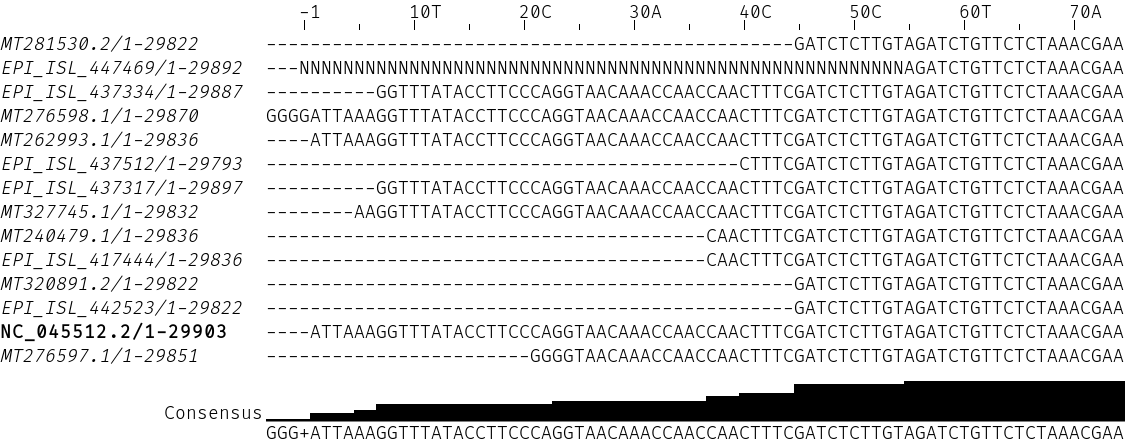
\includegraphics[width=1.3\linewidth]{jalview-clustal-start.png}}
  \caption{Differenze all'inizio dell'allineamento}
  \label{fig:jalview-start}

  \makebox[\textwidth][c]{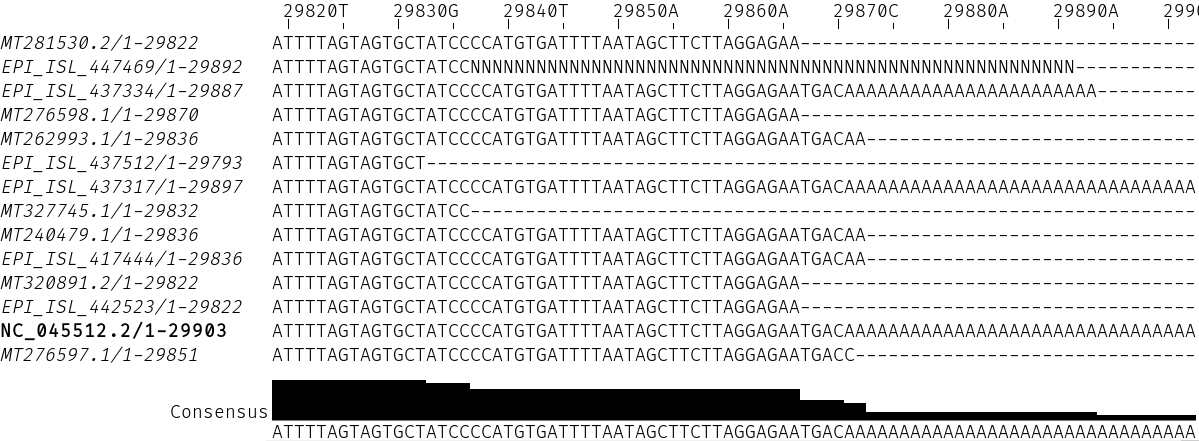
\includegraphics[width=1.3\linewidth]{jalview-clustal-end.png}}
  \caption{Differenze alla fine dell'allineamento}
  \label{fig:jalview-end}
\end{figure}

Inoltre, un paio di sequenze presentano basi mancanti o possibili problemi nel sequenziamento (\cref{fig:jalview-inner}).
Quest'ultimi verranno successivamente interpretate facendo riferimento allo IUPAC Code\footnote{\url{https://www.bioinformatics.org/sms/iupac.html}} e, specificatamente, verranno considerate come match rispetto al reference.

\begin{figure}[H]
  \makebox[\textwidth][c]{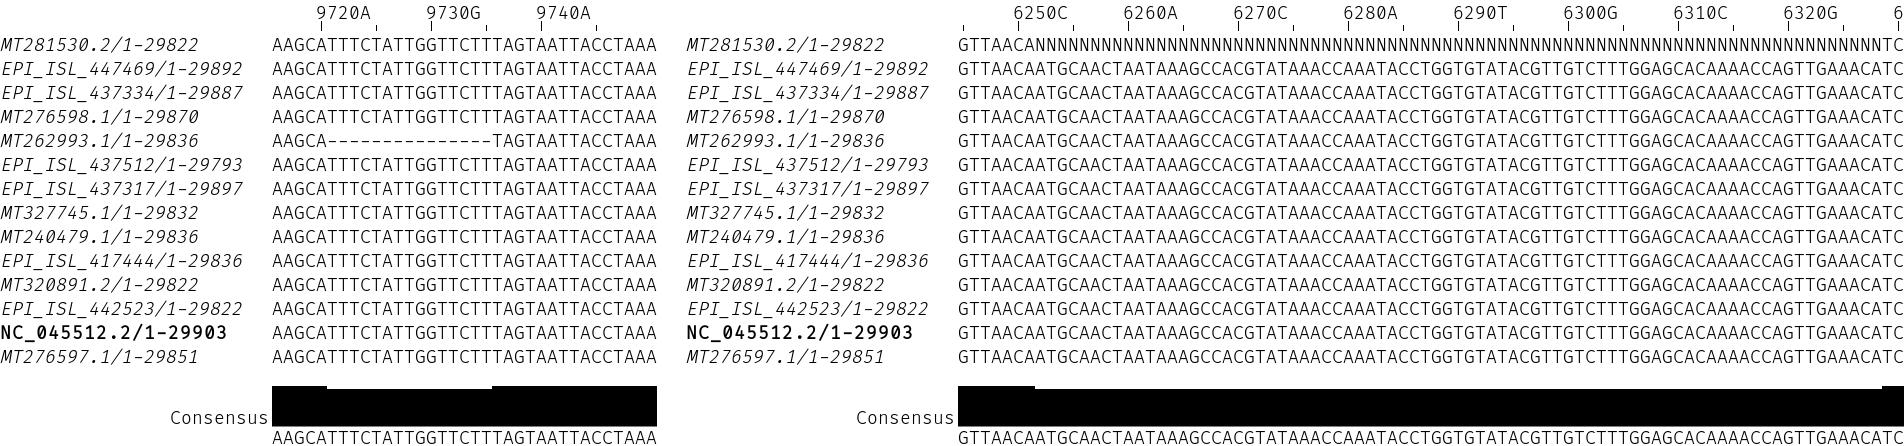
\includegraphics[width=1.5\linewidth]{jalview-clustal-inner.png}}
  \caption{Differenze all'interno dell'allineamento}
  \label{fig:jalview-inner}
\end{figure}


%BREVE DESCRIZIONE TOOLS?%
\section{Codice}
Il codice è in python ed esegue:
\begin{enumerate}
  \item pulisce la cartella di output per far spazio ai nuovi file, usando la libreria os.
  \item per ogni coppia di file in input contenendo l'analisi di allineamento eseguita usando i due tool:
  \begin{enumerate}
    \item salva il nome del file json in ooutput seguendo l'analisi.
    \item ne compara le differenze.
  \end{enumerate}
\end{enumerate}

\subsection{librerie}
\begin{itemize}
  \item\textbf{re:} usato in \textbf{parsers.py} per dividere ogni linea tra: [id\_sequenza, sequenza, posizioni] nelle funzioni di parsing.
  \item\textbf{hashlib:} usato in \textbf{utils.py} per creare l'hash da inserire come nome ai file JSON di output.
  \item\textbf{json:} usato in \textbf{utils.py} per elaborare ulteriormente l'uotput al fine di comparare i 2 tools di allineamento.
  \item\textbf{datetime:} usato in \textbf{utils.py} per prendere il tempo da inserire nell'hash, al fine di rendere unico l'output ed evitare sovrascritture.
  \item\textbf{os:} usato in \textbf{utils.py, main.py} per gestire input e output. Anche per pulire la cartella input nel main.
\end{itemize}

\subsection{descrizione metodi}
\begin{itemize}
  \item \lstinline{runClustal(inputFile, reference_id, nseq=3)}: funzione che esegue il parsing del file di allineamento clustal (inputFile), esegue il parsing degli allineamenti e li salva nel file di output. \newline nseq serve al parser in quanto la classe \lstinline{ClustalParser} richiede il numero di sequenze da elaborare nelle sue funzioni.

  \item \lstinline{runMuscle(inputFile, reference_id, nseq=3)}: funzione che esegue il parsing del file di allineamento muscle (inputFile), esegue il parsing degli allineamenti e li salva nel file di output. \newline

  \item \lstinline{parse(self, filename, reference=None, list=[]}:  legge il file in ingresso e restituisce il file in input suddiviso in: reference, sequenze, lunghezza sequenze. svolge la sua funzione sfruttando il metodo: \lstinline{parseLines(self, lines)}

  \item \lstinline{save(alignment, analyzer, reference_id=None, tool=None, path=None)}: crea file json di output chiamato reference\_id\_hash-sha1 del tempo di inzio esecuzione concatenato con sequences\_ids delle sequenze.

  \item \lstinline{jsonComp(file1, file2)}: funzione cre prende i 2 file json generati dall'elaborazione clustal e muscle e ritorna le differenze tra i 2 oggetti al fine di compararli.

  \item \lstinline{saveCompareFile(filename="differences.txt", country="", diff=[], path='output')}: file che divide per paese prende la lista di differenze tra gli allineamenti clustal e muscle e li aggiunge al file di output "differences.txt" per mostrarli.
\end{itemize}

\section{Output}
Come output vengono prodotti dei file json corrispondenti al nome reference\_seq\_hash.hexdigest(): l'id della reference accostata all'hash sha1 con encoding utf8 dell'id delle sequenze usate concatenate al tempo di inizio lavorazione (aggiunto per evitare di sovrascrivere l'output dello stessa serie di sequenze sia con muscle che con clustal).\newline
l'oggetto JSON è così composto:
\begin{lstlisting}
{
  "reference": reference_id,
  "analyzed_sequences":  id delle sequenze analizzate,
  "unmatches": {
    "(hash inizio mismatch + fine mismatch)": {
      "from": inizio mismatch,
      "to": fine mismatch,
      "sequences": sequenze contenenti la regione di mismatch
    }
  }
}
\end{lstlisting}

\section{Conclusioni}
Clustal tronca id troppo lunghi, i 2 tool di allineamento non sono identici, ...

\section{references}

\end{document}